\linespread{1.3}
\chapter{Dataset Curation, Proposed Approach and Specifications}

\section{Dataset Curation}
The development dataset is a novel dataset we curated using a subset of AudioSet. The development set contains both weakly-labelled and strongly-labelled data, as it incorporates the recently released strongly-labelled annotations for a subset of AudioSet \cite{hershey2021benefit}. This dataset is made up of 29,556 audio files in total, with 25,834 audio clips in the weakly-labelled train set, 2,380 clips in the strongly-labelled train set, 595 clips in the strongly-labelled validation set, and 747 clips in the strongly-labelled test set. There are a total of 25 sound event classes which are divided into two main categories: human and emergency. Most of the audio clips are 10 seconds long. The audio clips which are shorter than 10 seconds are padded with silence to 10 seconds. Table \ref{tab:main-dataset} lists the sound events and their statistics. The development set includes audio clips from the training set and validation set.\\

\begin{table}[!htp]
\centering
\begin{tabular}{|c|c|c|c|}
\hline
\multirow{2}{*}{\textbf{Sound Type}} & \multirow{2}{*}{\textbf{Sound Event}}                                                                                                                                                                                                                                                                               & \multicolumn{2}{c|}{\textbf{\begin{tabular}[c]{@{}c@{}}Number of \\ Event Instances\end{tabular}}}                                                                                                                                                                                                           \\ \cline{3-4} 
                                     &                                                                                                                                                                                                                                                                                                                     & \textbf{Development}                                                                                                                                                  & \textbf{Test}                                                                                                                        \\ \hline
Human                                & \begin{tabular}[c]{@{}c@{}}Applause\\ Breathing\\ Chatter\\ Cheering\\ Child speech, kid speaking\\ Clapping\\ Conversation\\ Cough\\ Crowd\\ Crying, sobbing\\ Female speech, woman speaking\\ Laughter\\ Male speech, man speaking\\ Run\\ Screaming\\ Shout\\ Sneeze\\ Walk, footsteps\\ Whispering\end{tabular} & \begin{tabular}[c]{@{}c@{}}552\\ 161\\ 259\\ 1,138\\ 2,119\\ 155\\ 1,004\\ 182\\ 2,220\\ 339\\ 4,263\\ 1,381\\ 10,739\\ 522\\ 243\\ 44\\ 279\\ 645\\ 460\end{tabular} & \begin{tabular}[c]{@{}c@{}}25\\ 31\\ 21\\ 35\\ 48\\ 25\\ 37\\ 26\\ 94\\ 21\\ 20\\ 59\\ 20\\ 20\\ 15\\ 11\\ 21\\ 30\\ 30\end{tabular} \\ \hline
Emergency                            & \begin{tabular}[c]{@{}c@{}}Air horn, truck horn\\ Car alarm\\ Emergency vehicle\\ Explosion\\ Gunshot, gunfire\\ Siren\end{tabular}                                                                                                                                                                                 & \begin{tabular}[c]{@{}c@{}}94\\ 140\\ 1,630\\ 466\\ 917\\ 2,889\end{tabular}                                                                                          & \begin{tabular}[c]{@{}c@{}}19\\ 37\\ 106\\ 16\\ 33\\ 160\end{tabular}                                                                \\ \hline
\end{tabular}
\caption{\label{tab:main-dataset}Summary of sound events in project dataset}
\end{table}

% This dataset was curated with the aid of the YouTube-DL and FFmpeg \cite{tomar2006converting} packages. YouTube-DL enables the audio clips to be downloaded from YouTube efficiently, while FFmpeg extracts a portion of the downloaded audio clips and resamples them to the predefined sample rate. 
The curation of the dataset was done in three main stages. In the first stage, we made a list of labels of the 25 sound event classes we wanted the audio clips extracted from AudioSet to be tagged as. Since the AudioSet sound event labels is a collection of sound events organised in a hierarchy, an audio clip tagged with a ‘child’ label would also be tagged with the ‘parent’ label. For instance, an audio clip tagged with the ‘Applause’ or ‘Cheering’ label is also tagged with the ‘Human group actions’ label. As such, we included the corresponding ‘parent’ labels to each of the 25 classes in the aforementioned list of labels. In the second stage, we filtered the publicly available metadata of the AudioSet dataset to extract the names of the audio clips that were only tagged with labels present in the list of labels produced in stage 1. In the final stage, we used YouTube-DL to download the audio clips whose names are present in the filtered metadata, and then used FFmpeg \cite{tomar2006converting} to trim the downloaded audio clips in accordance with the start and end time stated in the metadata, and resample them to 16k Hz.

\subsection{Dataset with Lower Audio Quality}
In real-life scenarios, the audio quality of a recording that a user typically inputs into the SED system would be quite poor. It would be unwise to assume that their input audio clips would always be of similar quality to the clips in the development dataset. Therefore, we created a development dataset with lower audio quality in order to develop a SED system that performs well with inputs of lower audio quality. This is done by using pipe and FFmpeg to generate different types of codec effects on the higher quality audio clips and resample them to 8k Hz. 

\section{Proposed Methodology}
In this thesis, we experimented with different system structures which incorporate the different approaches discussed in Chapter 2. The main development dataset used in this project is novel and the data type combination it consists of is slightly different from that of the standard SED datasets mentioned in Section 2.2. The project dataset consists of both weakly-labelled and strongly-labelled data, with the weakly-labelled training set being around 11 times larger than the strongly-labelled training set. This is in contrast to the standard datasets, which can be fully strongly-labelled (DCASE 2016) or weakly-labelled (DCASE 2017), weakly-labelled and unlabelled (DCASE 2018), or strongly-labelled, weakly-labelled and unlabelled (DCASE 2019 and DCASE 2020). As such, previous works based on these standard datasets were not entirely applicable to our task at hand. Therefore, we took ideas from each of these approaches, as well as proposed a frame-wise prediction pre-processing and post-processing method, in order to develop a system that was appropriate for the dataset we had to work with and the intended purpose of our SED system, which is to analyse clips with long audio duration.\\ 

With regards to the audio features, related works mentioned in Section 2.3 have shown that both log-mel and gammatone spectrograms are viable options to be used as input for training the SED systems. Both spectrograms were designed to better mimic the human auditory system. Thus, we experimented with both types of spectrogram representations in our SED system.\\

For data augmentation techniques, previous works mentioned in Section 2.4 focused on SpecAugment, time-shifting and mixup. Although there are other data augmentation techniques that may be useful for processing the spectrogram representations before passing them as input for training, previous works in \cite{kong2020sound, Miyazaki2020CONFORMERBASEDSE} have made use of the aforementioned techniques specifically for SED tasks, even producing the best-performing models for the DCASE 2017 and DCASE 2020 Task 4 challenges. Hence, we focused our experiments on these three data augmentation techniques for our SED system.\\ 

For model architectures, related works shown in Section 2.5 focused on GRU-based, transformer-based and conformer-based neural networks. As these networks have shown to produce comparative results in \cite{kong2020sound} and \cite{Miyazaki2020CONFORMERBASEDSE}, we experimented with the aforementioned network architectures for our SED system in order to determine the best one for our project development dataset.\\

According to \cite{kong2020sound}, rather than using manually-selected thresholds values, employing optimised threshold values determined from automatic threshold optimisation has been proven to improve the performance of SED systems. This is mainly because manually selected threshold values are rarely optimal and the optimal threshold value may be vastly different for different sound event classes. We thus employed the suggested method stated in \cite{kong2020sound} to implement automatic threshold optimisation in our SED system.\\

To address the issue regarding current SED systems, which is the lack of pre-analysis segmentation and the problems stemmed from processing only non-overlapping segments, as mentioned in Section 2.7, we implemented a pre-prediction audio clip segmentation step and post-prediction frame-wise prediction processing in the prediction system, which is further discussed in Section 3.5.

\section{System Architecture}
There are two main components of the SED system, which are namely the training system and prediction system. These systems are discussed in greater detail in the following subsections. 

\subsection{Training System}
The training system is the foundation for the development of our SED system. It is the system where most of the experiments are conducted. In this system, the audio clips in the training and validation sets are first packed into hdf5 files, and then transformed to their spectrogram representations. Next, data augmentation is applied on these spectrograms, which are then sent to the CNN-based models for training. Figure \ref{fig:training-system} shows the architecture of the training system.

\begin{figure}[!htb]
    \centering
    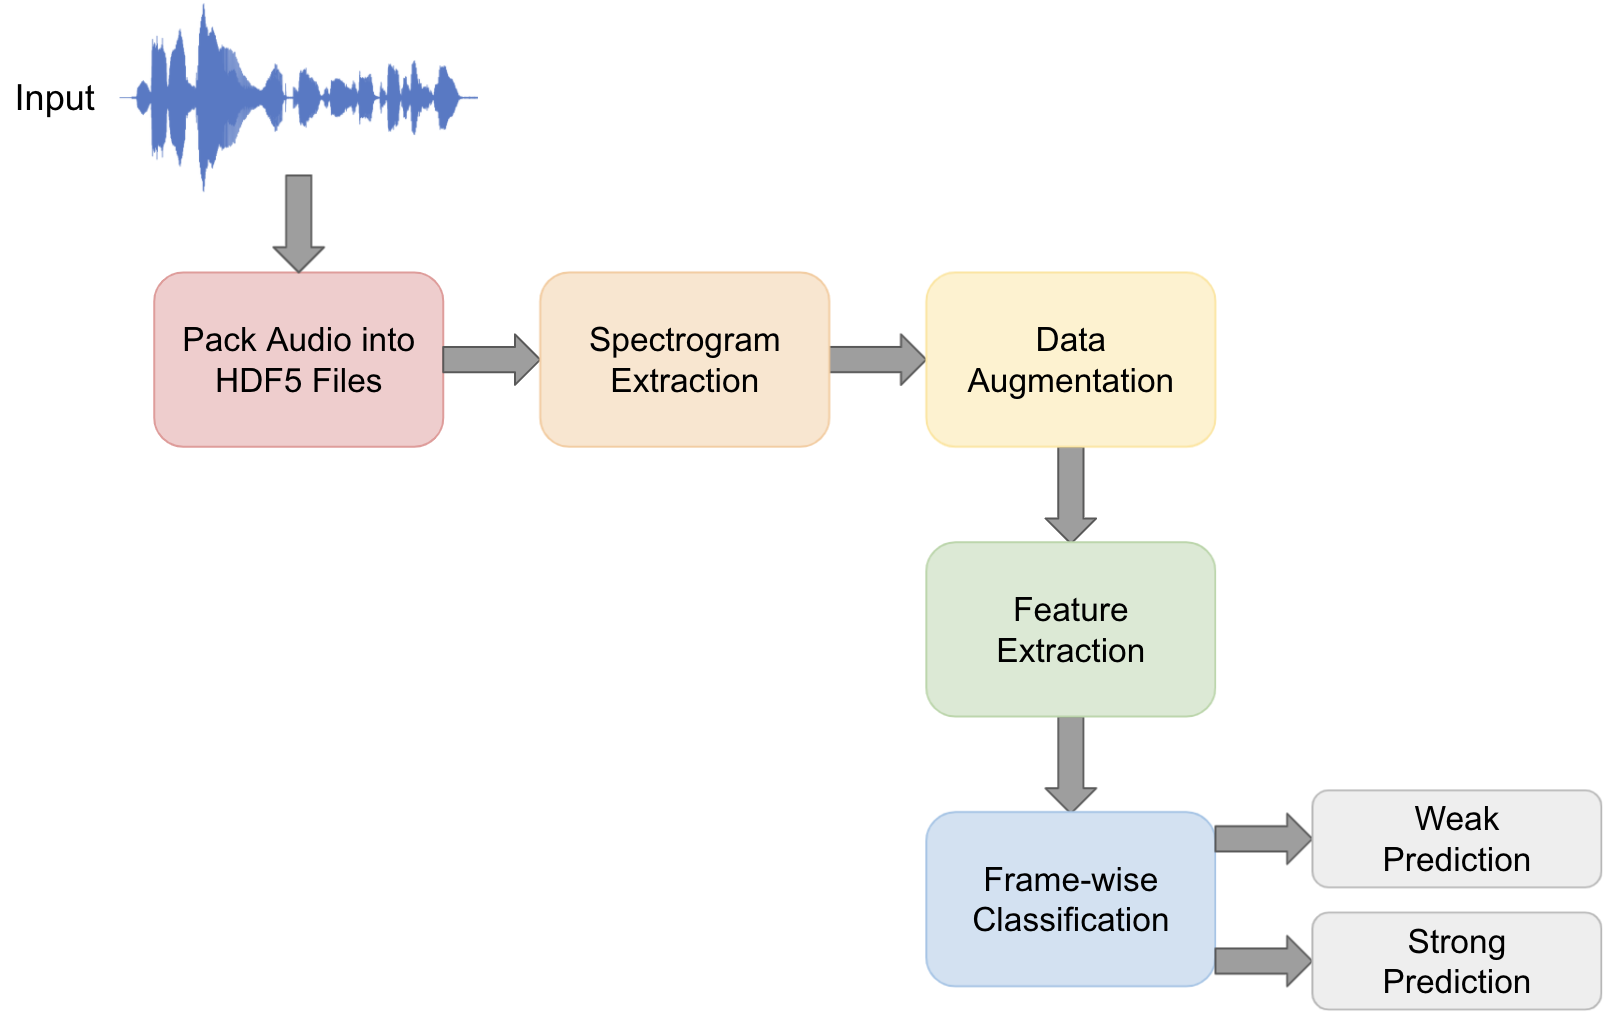
\includegraphics[width=\textwidth]{fig/training-system.png}
    \caption{Overview of training system}
    \label{fig:training-system}
\end{figure}

\subsection{Prediction System}
The prediction system implements the trained system from Section 3.3.1 and analyses audio input that is independent of the audio clips used in the training set and validation set. This system is used to experiment and determine the impact of applying the optimised thresholds, as well as segmenting audio clips before prediction and further processing after prediction. Figure \ref{fig:prediction-system} illustrates the structure of the prediction system.

\begin{figure}[!htb]
    \centering
    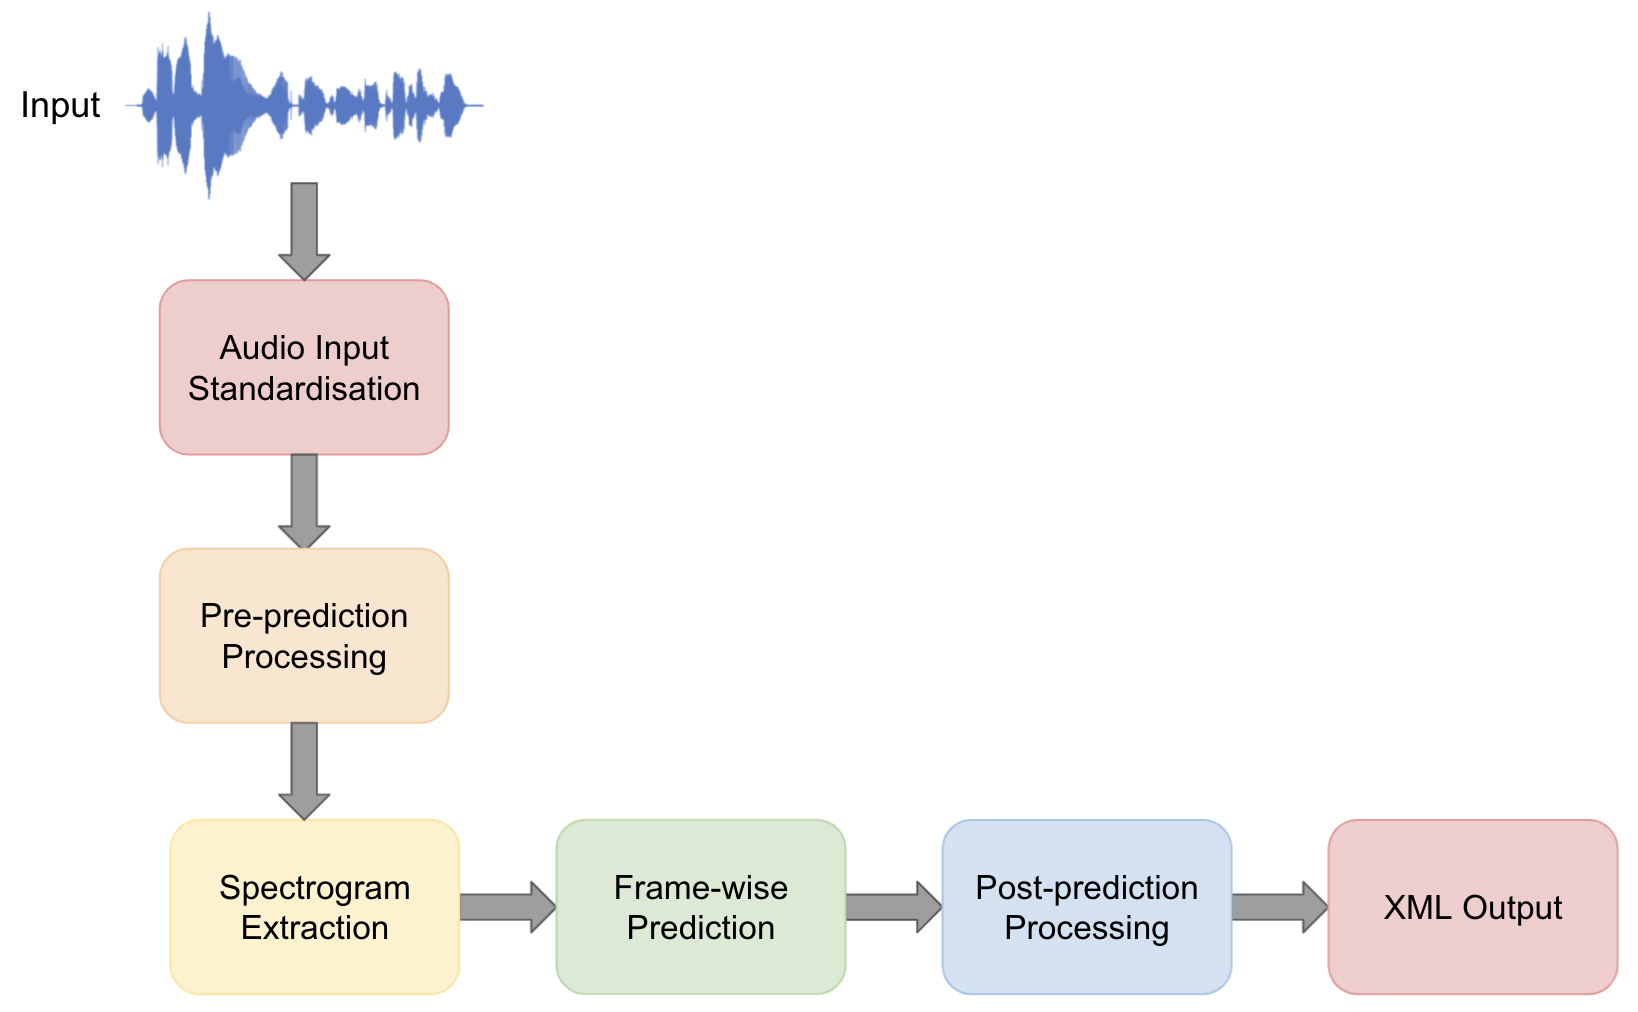
\includegraphics[width=\textwidth]{fig/prediction-system.png}
    \caption{Overview of prediction system}
    \label{fig:prediction-system}
\end{figure}

\section{Training System Specifications}
This section describes the components of the training system.

\subsection{Audio Input Packing}
The raw audio clip files from the dataset, in WAV format, are segmented into strongly-labelled training, weakly-labelled training, validation and testing sets. For each subset of the dataset, the waveforms are packed into a hdf5 file. This is mainly done to speed up training later on. 

\subsection{Spectrogram Extraction}
The process of extracting different spectrograms from the waveforms is specified in this section.

\subsubsection{Log-mel Spectrograms}
The packed waveforms are passed into the model in batches and their spectrogram representations are extracted. Next, the spectrograms are passed through a mel filterbank to generate mel spectrograms. Finally, a logarithmic operation is applied on the mel spectrograms to obtain log-mel spectrograms. This is done enitrely using Torchlibrosa, which uses GPU acceleration to speed up the process.

\subsubsection{Gammatone Spectrograms}
The process of extracting gammatone spectrograms from the packed waveforms is similar to that of extracting log-mel spectrograms, except it is passed through a gamma filterbank instead of a mel filterbank. Additionally, this process is not sped up using GPU. This is due to the unavailability of such a feature in the Torchlibrosa library.

\subsection{Data Augmentation}
For data augmentation, we employed time and frequency masking from SpecAugment \cite{specaugment}, as well as time-shifting \cite{timeshift} and mixup \cite{mixup}. 
For time-shifting, we randomly chose the frame-shift size by sampling from a Gaussian distribution, with a zero mean and a standard deviation of 90. For mixup, we randomly chose the \(\lambda\) value, as mentioned in equations \ref{eqn:mixup-1} and \ref{eqn:mixup-2}, by sampling from a beta distribution with \(\alpha\) = 0.1. Additionally, we experimented with different combinations of these data augmentation techniques, such as SpecAugment with mixup only, and SpecAugment with both time-shift and mixup. 

\subsection{Neural Network Model}
A CNN-based model is used as the feature extractor to extract the high level features from the spectrograms after data augmentation is applied. The output is then fed into a fully connected layer to do frame-wise classification to obtain the presence probabilities of the sound event classes over time steps.  We experimented with CNN-GRU (GRU here refers to a bidirectional GRU), CNN-Transformer and CNN-Conformer models, since they have achieved comparative performances in previous SED tasks \cite{kong2020sound, xu2017convolutional, Miyazaki2020CONFORMERBASEDSE}, as well as varied the number of convolutional layers used in the CNN portion. The CNN portion can be either modelled by a 9-layer or 14-layer CNN, which have shown to perform well on SED tasks \cite{kong2020sound, torchlibrosa}. Additionally, we experimented with transfer learning, using a pre-trained network as our feature extraction model. 

\subsubsection{CNN-Based Models}
The CNN-based model comprises of a CNN to capture local features, and an additional network, either a GRU, Transformer or Conformer, to capture the long-term temporal dependency. To construct the model, we first apply a CNN, either 9-layer or 14-layer, on the spectrogram in order extract the high level features. Next, the feature maps of the last convolutional layer are utilised to obtain embedding vectors along the time axis. The embedding can be denoted as \(x\) and has a shape of the number of time frames by the number of channels. These embeddings are then passed into the network that captures the long-term temporal dependency, which can be either a GRU, Transformer or Conformer, in order to obtain the output features. A fully connected layer with sigmoid activation is applied then on this output to predict the presence probabilities of sound event classes over time steps.

% \subsubsection{CNN-GRU}
% As mentioned in Section 2.5.2, there a few types of CRNNs we can consider to implement to tackle a SED task. For this thesis, we focus on the CNN-GRU since the performance of GRUs are on par with LSTMs, but are computationally more efficient \cite{chung2014empirical}. To construct the CNN-GRU, we first apply a CNN, either 9-layer or 14-layer, on the spectrogram in order extract the high level features. Next, the feature maps of the last convolutional layer are utilised to obtain embedding vectors along the time axis. The embedding can be viewed as \(x\) with a shape of the number of time frames by the number of channels. These embeddings are then passed into the GRU in order to obtain the output features. A fully connected layer with sigmoid activation is applied on this output to predict the presence probabilities of sound event classes over time steps.

% \subsubsection{CNN-Transformer}\\[0.1in]
% %For SED, the input is usually a time-frequency representation such as a log-mel spectrogram. A spectrogram is a low level feature and CNNs have been proposed to apply on the spectrogram representations to extract high level features \cite{cnn-at}. 
% To build the CNN-Transformer system, a CNN, either 9-layer or 14-layer, is applied on the spectrogram representation of an audio clip, followed by a transformer block. Convolutional layers in the CNN are used to extract high level features of the input spectrograms. We use the feature maps of the last convolutional layer to obtain embedding vectors along the time axis, whcih are then fed as input to the transformer. The embedding can be viewed as \(x\) with a shape of the number of time frames by the number of channels. The output of the transformer has a shape of \(T \times d_v\). A fully connected layer followed by a sigmoid non-linearity is applied on this output to predict the presence probabilities of sound classes over time steps. 
% %An aggregation function such as average aggregation can be applied to average out those probabilities along the time domain to obtain the weakly-labelled result. This is an important function as this result is used for training the weakly-labelled train set, which makes up a large portion of the entire train set.

% \subsubsection{CNN-Conformer}\\[0.1in]
% %Similar to the CNN-Transformer, the input is typically a time-frequency representation such as a log-mel spectrogram. 

% Similar to the CNN-GRU and CNN-Transformer, the CNN-Conformer system is constructed by applying a CNN described in Section 2.6.1 on the spectrograms of the audio input. The CNN is used to extract high level features of the input spectrograms. The feature maps of the last convolutional layer are utilised to obtain embedding vectors along the time axis. The embedding can be viewed as x with a shape of the number of time frames by the number of channels. These embeddings are then passed into the conformer block to generate the output features. A fully connected layer with sigmoid activation is applied on this output to predict the presence probabilities of sound classes over the time steps. %Like the CNN-Transformer, aggregation functions such as average aggregation can then be applied to average out those probabilities along the time domain to obtain the weakly-labelled result. This result is used for training the weakly-labelled subset of the train set.

\subsubsection{Transfer Learning}
As discussed in Section 2.5.5, there are two main transfer learning strategies we can apply. In our approach, we only focus on the second strategy, which is to fine-tune the pre-trained model on the project dataset. This involves transferring the weights from a pre-trained CNN, and then fine tuning the network using the new target data. In this thesis, we used the VGGish \cite{vggish} pre-trained model to conduct transfer learning. VGGish is a CNN model from Google that has been pre-trained on the YouTube-8M dataset. The architecture of this network is inspired by the famous VGG \cite{vgg} networks used for image classification. In our experiment, we used VGGish as a feature extractor, fine-tuned on our project dataset, to obtain the output features of an input spectrogram. These output features would later be fed into a classifier, which is a fully connected layer with sigmoid activation to predict the presence probabilities of sound event classes over the time steps.

\subsection{Clip-wise Training}
The clip-wise training method involves feeding entire audio clips as training input, instead of segmenting them beforehand. As such, this method does not explicitly assign tags for each frame \(x_m\). It learns the tags of \(x_m\) implicitly instead from the hidden layer of a neural network. The frame-wise prediction of a frame \(x_m\) can be denoted as \(f(x_m)\). Then, the prediction on an audio clip \(X\) can be obtained by aggregating the frame-wise predictions. This is done to obtain the weakly-labelled result, which is used for training the weakly-labelled subset of the train set. The aggregation can be an average or attention function over the prediction of all frames of each sound event class \(k\). The average function can be defined as:
\begin{equation}
F(X)_k = \sum^M_{m=1}f(x_m)_k .
\end{equation}
% To apply the average function, we include an additional fully-connected layer with sigmoid activation in the network.

To employ the attention function, an additional feed-forward neural network with softmax activation is introduced to infer the temporal locations of each occurring sound event class. In order to preserve the time resolution of the input whole audio spectrogram, we adjust the pooling steps in the CNN-based models by only pooling on the spectral axis while not pooling on the time axis. The feed-forward with sigmoid activation does classification at each frame, while the feed-forward with softmax activation attends to the most important frames for each sound event class. The attention function can be concisely defined as:
\begin{equation}
F(X)_k = \sum^M_{m=1}f(x_m)_k p(x_m)_k ,
\end{equation}
where \(p(x_m) = \frac{exp(w(x_m)_k)}{\sum^M_{j=1}exp(w(x_j)_k)}\), and \(w(\cdot)\) is a linear transformation.\\

As there are two types of data in the development dataset, which are namely the weakly-labelled training set and strongly-labelled training set, each input batch contains a 3 to 1 ratio of the weakly-labelled and strongly-labelled data respectively. We therefore have two different methods of calculating the loss between the predictions and the ground truth for these two types of data.  For the weakly-labelled training set, we calculate the categorical binary loss between the clip-level prediction \(F(X)\) and the weak ground truth label of \(X\) as:
\begin{equation}
E = -\sum^K_{k=1}[y_k\log{F(X)_k} + (1 - y_k)log(1 - F(X)_k)] .
\end{equation}

For the strongly-labelled training set, we calculate the categorical binary loss between the frame-wise prediction \(f(x_m)\) and the strong ground truth of \(X\) as:
\begin{equation}
E = -\sum^M_{m=1} \sum^K_{k=1}[y_k\log{f(x_m)_k} + (1 - y_k)log(1 - f(x_m)_k)],
\end{equation}

where \(y \in \{0, 1\}^K\) represents the tag of each frame, with \(K\) denoting the number of sound event classes. Finally, we sum the weak and strong losses together, which is then used as the main loss function to minimise when training the overall model.

\subsection{Automatic Threshold Optimisation}
In this step, we first optimize the systems and evaluate them based on the metrics that do not depend on the thresholds such as mean average precision (mAP). Next, for a trained system, we optimize the thresholds over a specific metric such as F1-score. To do so, we followed the steps below:

\begin{enumerate}
    \item Initialise thresholds \(\Theta\), where \(\Theta\) consists of the thresholds for each of the sound event classes.
    \item Obtain predictions for each audio clip by applying \(\Theta\).
    \item Initialise loss function J, which is based on negative F1-score. The reason for using such a metric is because minimizing negative F1-score is equivalent to maximising F1 score.
    \item Calculate the gradient of each parameter \(\theta_k\) in \(\Theta\) using the following formula:
    \begin{equation}
    \nabla_\theta J(\Theta) = \frac{J(\Theta + \delta\Theta) - J(\Theta)}{\delta\theta} ,    
    \end{equation}
    \item Apply gradient descent \cite{ruder2016overview} after calculating the numerical gradient of all parameters to obtain optimised thresholds \(\Theta_{opt}\). Gradient descent optimisation can be denoted as:
    \begin{equation}
    \Theta \leftarrow \Theta - \alpha \nabla\Theta J ,
    \end{equation}
    where \(\alpha\) denotes the learning rate.
    The Adam optimiser \cite{kingma2017adam} is then used to optimise J(\(\Theta\)) due to its fast convergence.
\end{enumerate}

% A more concise explanation of the automatic threshold optimisation algorithm is shown in Algorithm 3.1 below.

\section{Prediction System Specification}

\subsection{Audio Input Standardisation}
An audio clip recording of any format can be passed into the system, but those that are not in WAV format will be automatically converted from their original format to WAV. This is done using the FFmpeg package.

\subsection{Pre-Prediction Segmentation and Frame-wise Class Predictions}
The pre-prediction segmentation step involves segmenting the input audio clip into segments of x seconds before passing them into the trained system to obtain the frame-wise class predictions. 
% This pre-prediction processing method has not been used in previous works on SED. 
In this approach, we apply a \(x\) second rolling window with a \(y\) second stride on an audio clip. The values of \(x\) and \(y\) are tuned according to the F1-score of the validation set, which was done using a grid search method \cite{lavalle2004relationship}. We initialised a set of possible rolling window values as \(X\), where \(X\) ranges from 2 to 10, with a step of 0.5, and a set of possible stride values as \(Y\), where \(Y\) ranges from 0.5 to 1.5, with a step of 0.5.\\ 

By applying a rolling window and sending these portioned segments of the audio clip to the trained system to be predicted on individually, some segments may be overlapped. The number of overlaps varies based on the position of the segment on the time axis. For instance, if we apply a 5 second rolling window with a 1 second stride on an audio clip, the maximum number of overlaps a segment can have is 4, while the minimum is 0. An illustration, Figure \ref{fig:overlap}, is shown below to provide a clearer explanation on the varying number of overlaps for each segment in a 14-second long audio clip.

\begin{figure}[!htb]
    \centering
    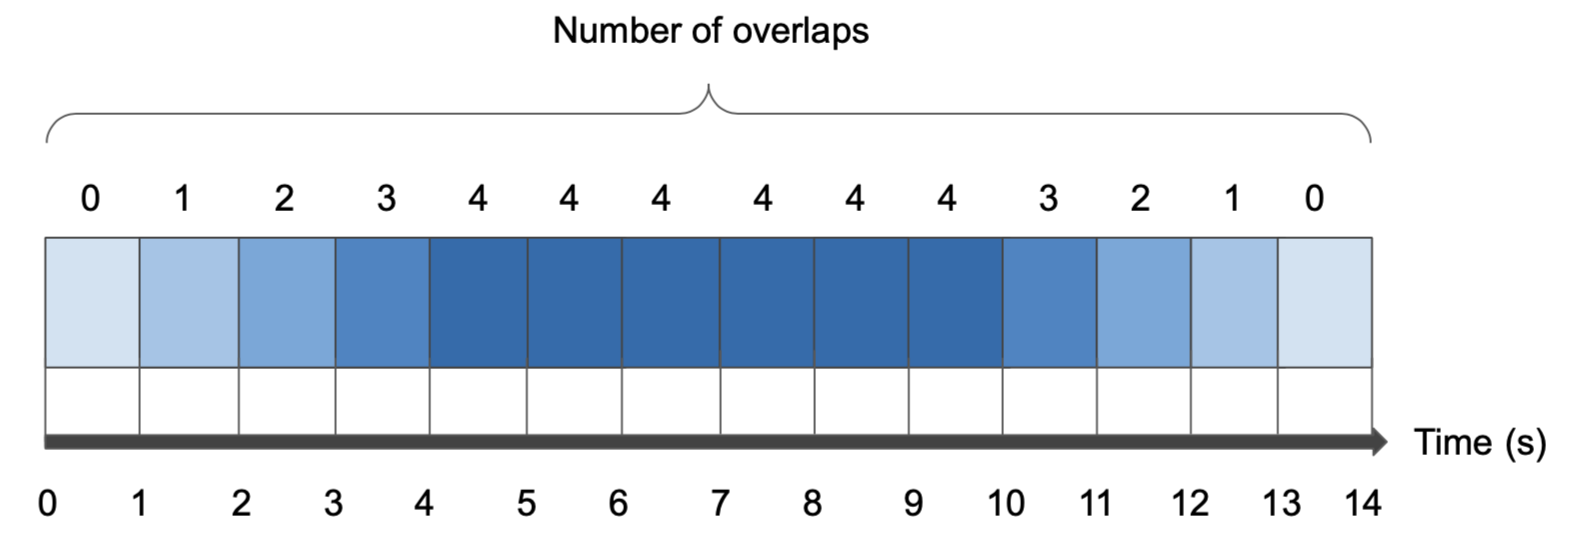
\includegraphics[width=\textwidth]{fig/overlap.png}
    \caption{Example of prediction overlap}
    \label{fig:overlap}
\end{figure}

\subsection{Post-Prediction Processing}
The post-prediction processing step involves manipulating the frame-wise predictions summed across the segments which were overlapped. As shown in Figure 3.3, the number of overlaps differs for each segment as it is dependent on the position of the segment on the time axis. In this thesis, we have proposed two methods of amalgamating the predictions, which is to 1) average the frame-wise predictions or 2) implement a voting scheme.   

\subsubsection{Averaging Frame-wise Predictions}
In this method we first sum the frame-wise predictions together and then average them based on the number of overlaps present in a particular segment. Once the averaged frame-wise predictions are obtained, we apply a set of thresholds, such as the optimised thresholds, over them to determine which sound events are present in which frames. If sequential frames are detected to contain a certain sound event, we determine the onset and offset times of the sound event to correspond to the first and last frames in the sequence, respectively.

\subsubsection{Voting Scheme}
This method involves using a set of thresholds, such as the optimised thresholds, to determine the presence of a sound event. If present, a numerical value of 1 is assigned to the frame for that particular sound event, otherwise 0 is assigned. Next, we sum the binarized frame-wise predictions together and then threshold based on the number of overlaps present in each particular segment. This is done to determine which sound events are present in which frames. Similar to the preceeding method, if sequential frames are detected to contain a certain sound event, we determine the onset and offset times of the sound event to correspond to the first and last frames in the sequence, respectively.

% The post-prediction processing step involves manipulating the frame-wise predictions summed across the segments which were overlapped. In this thesis, we have proposed a method of doing so, which is to average the frame-wise predictions based on the number of overlaps present in a particular segment. As shown in Figure 3.3, the number of overlaps differs for each segment as it is dependent on the position of the segment on the time axis. Once the averaged frame-wise predictions are obtained, we apply a set of thresholds over them to determine which sound events are present in which frames. If sequential frames are detected to contain a certain sound event, we determine the onset and offset times of the sound event to correspond to the first and last frames in the sequence, respectively.

\subsection{Prediction Output Format}
Once we have determined the onset and offset times of the sound events present in an audio clip, we compile them and output them in a XML style format. Figure \ref{fig:xml-output} shows an example of the output of our prediction system.

\begin{figure}[!htb]
    \centering
    \begin{lstlisting}[language=XML]
<AudioDoc name="audio_filename">
    <SoundCaptionList>
        <SoundSegment stime="0.32" duration="9.76">Applause</SoundSegment>
        <SoundSegment stime="0.48" duration="0.96">Cheering</SoundSegment>
        <SoundSegment stime="3.88" duration="5.84">Cheering</SoundSegment>
                                .
                                .
                                .
        <SoundSegment stime="464.32" duration="1.96">Male_speech_man_speaking</SoundSegment>
        <SoundSegment stime="473.16" duration="0.40">Clapping</SoundSegment>
        <SoundSegment stime="473.32" duration="0.68">Male_speech_man_speaking</SoundSegment>
    </SoundCaptionList>
</AudioDoc>
    \end{lstlisting}
    \caption{Prediction system output}
    \label{fig:xml-output}
\end{figure}

\section{Tools and Technologies}
This section summarises the tools and packages used in the development of the SED system.

\subsection{Environment Setup}
Table \ref{tab:env} below provides an overview of the environment setup of this project.

\begin{table}[!htp]
\centering
\begin{tabular}{|c|c|}
\hline
\textbf{Hardware}         & NVIDIA Tesla V100 32 GB \\ \hline
\textbf{Operating System} & Linux                   \\ \hline
\end{tabular}
\caption{\label{tab:env}Environment setup}
\end{table}

\subsection{Language and Libraries}
The SED system was created with a combination of different libraries. Table \ref{tab:tools-libraries} below provides a summary of tools and technologies used in this project. The source code of this project is written entirely in Python.

\begin{table}[!htp]
\centering
\begin{tabular}{|c|c|}
\hline
\textbf{Component}                                                                                                                                                                           & \textbf{Libraries}                                                                                                     \\ \hline
\begin{tabular}[c]{@{}c@{}}Project dataset curation\\ Audio input packing\\ Spectrogram transformation\\ System training\\ Audio input standardisation\\ Performance evaluation\end{tabular} & \begin{tabular}[c]{@{}c@{}}YouTube-DL, FFmpeg\\ HDF5\\ TorchLibrosa, NumPy\\ PyTorch\\ FFmpeg\\ sed\_eval\end{tabular} \\ \hline
\end{tabular}
\caption{\label{tab:tools-libraries}Tools and Libraries used}
\end{table}

\subsubsection{Python}
Python \cite{python} is a programming language predominantly used for this project due to the existing libraries that are useful for developing the SED system. For example, libraries such as PyTorch, which is discussed further in Section 3.6.2.2, is the foundation of our project as we used it to build and train models we experimented with in this thesis. 

\subsubsection{PyTorch}
PyTorch \cite{NEURIPS2019_9015} is a Python package that provides high-level features such as tensor computation with strong GPU acceleration, and deep neural networks built on a tape-based auto-grad system. We used this package to build the models we experimented with in this thesis, as well as speed up training by using a GPU alongside it. 

\subsubsection{FFmpeg}
FFmpeg \cite{tomar2006converting} is a command line program for transcoding multimedia files. It is a very fast video and audio converter that can also collect data from a live audio/video source. It can also convert between arbitrary sample rates and resize video on the fly with a high quality polyphase filter. We used this program to standardise the input audio files to WAV format in the prediction system.

\subsubsection{Librosa}
Librosa \cite{brian_mcfee_2021_4792298} is a Python package for music and audio analysis. It provides the building blocks necessary to create music information retrieval systems. It provides functions to load and resample audio files, and to transform waveforms to different audio feature representations.

\subsubsection{TorchLibrosa}
TorchLibrosa \cite{torchlibrosa} is a PyTorch implementation of some librosa functions to transform raw waveforms to spectrograms with GPU acceleration. It provides almost identical features to the standard librosa functions, with numerical difference less than 1e-5. However, it is limited in its usage as it can only generate log-mel spectrograms as of late.

\subsubsection{YouTube-DL}
YouTube-DL is a command-line program to download audio and videos from YouTube.com and over one thousand other video hosting websites. We used this library to download the corresponding subset of AudioSet audio files from YouTube in order to curate our project dataset.

\subsubsection{sed\textunderscore{eval}}
sed\textunderscore{eval} \cite{sed-eval} is an open source Python toolbox which provides a standardized, and transparent way to evaluate sound event detection systems. This toolbox has been used as the main evaluation function for all the SED DCASE challenges.

\subsubsection{HDF5}
HDF5 \cite{hdf5} is a data software library and file format that is used to manage, process, and store heterogeneous data. It is built for fast I/O processing and storage. We used this library to store our data in order speed up the training and evaluation processes.

%=== END OF PROPOSED APPROACH ===
\newpage